
\documentclass[8pt,a4paper]{report}
\usepackage[latin1]{inputenc}
\usepackage{amsmath}
\usepackage{amsfonts}
\usepackage{amssymb}
\usepackage{graphicx}
\usepackage{hyperref}
\usepackage{multicol}
\usepackage[margin=0.4in]{geometry}
\usepackage{karnaugh-map}
\usepackage{amsthm}
\usepackage{mathtools}
\usepackage{listings}
\newcommand{\myvec}[1]{\ensuremath{\begin{pmatrix}#1\end{pmatrix}}}
\let\vec\mathbf
\begin{document}

\raggedright{
\includegraphics[scale=0.8]{iith.png}} \hspace{12cm}\raggedleft FWC22084\vspace{8mm}\\ 

\centering \Large \textbf{ASSIGNMENT- MATRICES}
\\ \centering \Large \textbf{CONICS} \vspace{15mm}

\begin{multicols}{2}


\raggedright \Large \textbf{Contents} \vspace{2mm}
\begin{itemize}
\raggedright \item Problem \item Solution\item Construction
\end{itemize}\vspace {5mm}
 

\raggedright \Large \textbf{Problem:} \vspace{2mm}
	\\  If the line $y = mx+7\sqrt{3}$ is normal to the hyperbola $\frac{x^2}{24}-\frac{y^2}{18} =1$,then the value of m is:\vspace{4mm}
\\\raggedright\Large \textbf{Solution:} \vspace{2mm}
	\\ \raggedright The equation of given hyperbola is \centering $\vec{x^{\top}}\vec{V}\vec{x} +2\vec{u^{\top}}\vec{x} + \vec{f} = \textbf{0}$ \\ 
\raggedright where\begin{align}
    \vec{V} = \myvec{\frac{1}{24}&0\\0&-\frac{1}{18}}\\
    \vec{u} = \myvec{0\\0}\\
    \vec{f} = -1
\end{align}
\raggedright The equation of the normal is\\ \centering$\vec{n^{\top}}\vec{x} = \textbf{C}$\\
 \raggedright whose normal vector is \\ \centering$\vec{n} = \myvec{-m\\1} , \textbf{C} = 7\sqrt{3}$\\
\raggedright Let us consider a tangent perpendicular to given normal with normal vector $\vec{n_t}$, \\
\centering $\vec{n_t} = \myvec{1\\m} $\\
\raggedright   Given the normal vector $\vec{n_t}$, the tangent points of contact to conic are given by\\
\begin{align}
\vec{q}_i &= \vec{V}^{-1}(\kappa_i \vec{n}_t-\vec{u}), i = 1,2\\
\text{where }\kappa_i &= \pm \sqrt{\frac{f_0}{\vec{n}_t^{\top}\vec{V}^{-1}\vec{n}_t}}
\end{align}
\raggedright Substituting points of contact of tangent(eq 4) in the normal equation ,
\begin{align*}
 \vec{n}^{\top}(\vec{q}_i) = \textbf{C}\\
 \vec{n}^{\top}(\vec{V}^{-1}(\kappa_i \vec{n}_t-\vec{u}) )= 7\sqrt{3}
 \vec{u}= \myvec{0\\0} ,\\
 \vec{n}^{\top}(\vec{V}^{-1}\kappa_i \vec{n}_t )= 7\sqrt{3}\\
 \kappa_i(\vec{n}^{\top}\vec{V}^{-1}\vec{n}_t) = 7\sqrt{3}\\
\kappa_i\myvec{-m&1}\myvec{-24\times18}\myvec{\frac{-1}{18}&0 \\ 0&\frac{1}{24}}\myvec{1\\m} = 7\sqrt{3}\\
 \kappa_i\myvec{-24\times18}\myvec{\frac{1}{18}&\frac{m}{24}}\myvec{1\\m} =7\sqrt{3}\\
\kappa_i\myvec{-24\times18}\myvec{\frac{m}{18}+\frac{m}{24}} =7\sqrt{3}\\
 \kappa_i\myvec{-24\times18}\myvec{\frac{42m}{24*18}} =7\sqrt{3}\\
\end{align*}
	\begin{align}-\kappa_i m = \frac{\sqrt{3}}{6}\end{align}
\raggedright  Value of $\kappa_i$:\\
\begin{gather*}
      \kappa_i = \pm \sqrt{\frac{f_0}{\vec{n}_t^{\top}\vec{V}^{-1}\vec{n}_t}}\\
           f_0  = \vec{u}^{\top}\vec{V}^{-1}\vec{u}-f \\
                f_0 = -f\\
             \kappa_i  = \pm \sqrt{\frac{1}{ \vec{n}_t^{\top}\vec{V}^{-1}\vec{n}_t}}\\
\kappa_i = \pm \sqrt{\frac{1}{\myvec{-24\times18}\myvec{ 1&m}\myvec{\frac{-1}{18}&0\\0&\frac{1}{24}}\myvec{1\\m}}}\\
   \kappa_i = \pm\frac{1}{6}\sqrt{\frac{1}{-12\myvec{\frac{-1}{18}&\frac{m}{24}}\myvec{1\\m}}}\\
\kappa_i = \pm\frac{1}{6}\sqrt{\frac{1}{-12\myvec{-\frac{1}{18}+\frac{m^2}{24}}}}\\
\kappa_i = \pm\frac{1}{6}\sqrt{\frac{1}{-2\myvec{-\frac{1}{3}+\frac{m^2}{4}}}}
\end{gather*}
\raggedright Substituting value of $\kappa_i$ in eq 6,
\begin{align*}
  -\kappa_i m = \frac{\sqrt{3}}{6}
\pm\frac{1}{6}\sqrt{\frac{1}{-2\myvec{-\frac{1}{3}+\frac{m^2}{4}}}} m= \frac{\sqrt{3}}{6}\\
\pm\sqrt{\frac{1}{2\myvec{-\frac{1}{3}+\frac{m^2}{4}}}} m= \sqrt{3}
\end{align*}
\raggedright Squaring on both sides,
\begin{align*}
\frac{m^2}{\frac{2}{3}-\frac{2m^2}{4}} = 3\\
m^2 = 2 - \frac{3m^2}{2}\\
\frac{5m^2}{2} = 2\\
 m =\pm\frac{2}{\sqrt{5}}
\end{align*}
\raggedright\Large \textbf{Construction:} \vspace{2mm}
The input parameters for this construction are 
\begin{center}
\begin{tabular}{|c|c|}
	\hline
	\textbf{Symbol}&\textbf{Value}\\
	\hline
	n&$\
	\begin{pmatrix}
		-\frac{2}{\sqrt{5}}\\
		1\\
	\end{pmatrix}$%
	\\
	\hline
	V&$\
	\begin{pmatrix}
		\frac{1}{24}&0\\
		0&-\frac{1}{18} \\
	\end{pmatrix}$%
	\\
	\hline
	u&$\
	\begin{pmatrix}
		0\\
		0\\
	\end{pmatrix}$%
	\\
	\hline
	q&$\
	\begin{pmatrix}
		0\\
		7\sqrt{3}\\
	\end{pmatrix}$%
	\\
	\hline
	C1& 7$\sqrt{3}$
	\\
	\hline
	f&-1\\
	\hline
\end{tabular}
\end{center}
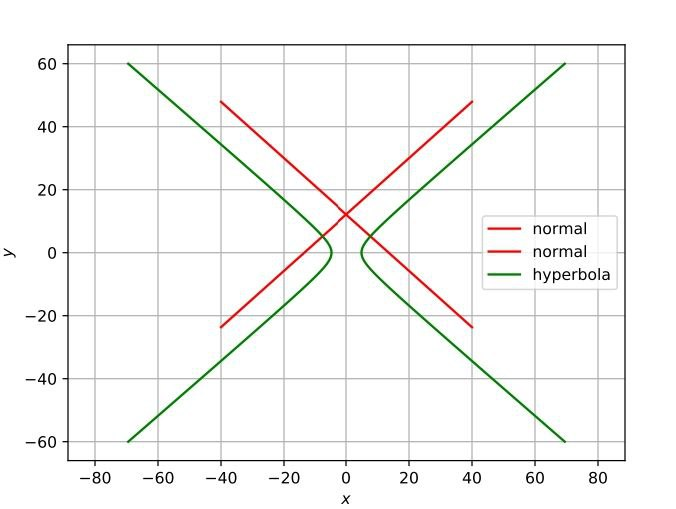
\includegraphics[scale=0.4]{hyp.jpg}
The below python code realizes the above construction:	
\centering     https://github.com/reshma0639/FWC-Assignment-1/blob/main/matrices/line.py
\end{multicols}
\end{document}
